1. Exprese \( D \subset \mathbb{R}^{2} \) como una región Tipo I y Tipo II. Después resuelva las dos integrales, esto es, en la región Tipo I y en la región Tipo II. Finalmente dibuje las regiones de integración. \\
a) \( \iint_{D} x d A \) donde \( D \) esta encerrada por las rectas \( y=x, y=0 \) y \( x=1 \).
Para una región Tipo I, la región D se describe como \( D = \{ (x, y) \mid a \leq x \leq b, g_{1}(x) \leq y \leq g_{2}(x) \} \).

\( x \) varía desde \( 0 \) hasta \( 1 \) (por las rectas \( y = x \) y \( x = 1 \)). \\
\( y \) varía desde \( 0 \) hasta \( x \) (por las rectas \( y = 0 \) y \( y = x \)). \\

Entonces, la región Tipo I es:
\[
D = \{(x, y) \mid 0 \leq x \leq 1, 0 \leq y \leq x\}
\]
La integral es:
\[
\iint_{D} x \, dA = \int_{0}^{1} \int_{0}^{x} x \, dy \, dx
\]
Separamos la integral doble en un producto de dos integrales (recordemos que esto es aplicable cuando tienes una función integrada respecto de $x$ y $y$ $f(x,y)=g(x)h(y)$). En tanto y se tiene,
\[
   \int_{0}^{x} x \, dy = x \cdot y \bigg|_{0}^{x} = x^2
   \]

Ahora con respecto a x:
\[
   \int_{0}^{1} x^2 \, dx = \left[\frac{x^3}{3}\right]_{0}^{1} = \frac{1}{3}
   \]

Por otra parte para una región Tipo II, la región D se describe como \( D = \{ (x, y) \mid c \leq y \leq d, h_{1}(y) \leq x \leq h_{2}(y) \} \). Aquí \( y \) varía desde \( 0 \) hasta \( 1 \) en tanto $x$ varía desde $y$ hasta 1.

Entonces, la región Tipo II es:
\[
D = \{(x, y) \mid 0 \leq y \leq 1, y \leq x \leq 1\}
\]

La integral para esta región es:
\[
\iint_{D} x \, dA = \int_{0}^{1} \int_{y}^{1} x \, dx \, dy
\]

Usamos la misma propiedad de separar como un producto de integrales. Veamos que para $x$:
\[
   \int_{y}^{1} x \, dx = \left[\frac{x^2}{2}\right]_{y}^{1} = \frac{1}{2} - \frac{y^2}{2}
   \]
Con respecto a $y$ se tiene.
\[
   \int_{0}^{1} \left(\frac{1}{2} - \frac{y^2}{2}\right) \, dy = \left[ \frac{y}{2} - \frac{y^3}{6} \right]_{0}^{1} = \frac{1}{2} - \frac{1}{6} = \frac{1}{3}
   \]

\begin{figure}[h]
    \centering
    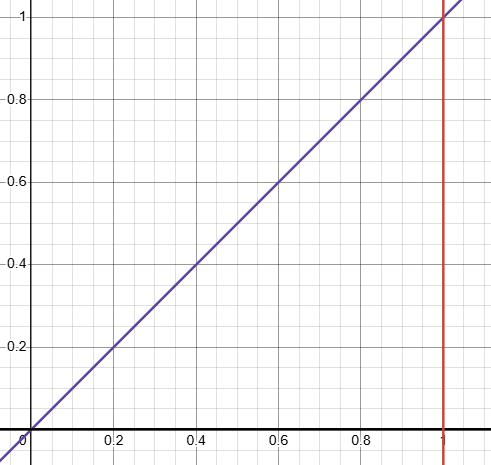
\includegraphics[width=0.5\linewidth]{1a.png}
    \caption{Región de integración a)}
    \label{fig:enter-label}
\end{figure}

b) \( \iint_{D}|x y| d A \) donde \( D \) esta encerrada por las curvas \( y=x^{2} \) y \( y=3 x \). \\

Para expresar D como una región Tipo I y Tipo II, primero identificamos las curvas $y=x^2$ y $y=3x$, que se intersectan en $x=0$ y $x=3$ ($x^2 - 3x = 0 \implies x(x - 3) = 0$).
Región Tipo I: \( D \) es el conjunto de puntos \((x, y)\) tal que \( 0 \leq x \leq 3 \) y \( x^2 \leq y \leq 3x \). La integral se describe como sigue.
\[
\int_{0}^{3} \int_{x^2}^{3x} |xy| \, dy \, dx
\]
Región Tipo II: D es el conjunto de puntos (x,y) tal que \( 0 \leq y \leq 9 \) y \( \sqrt{y} \leq x \leq \frac{y}{3} \). La integral es:
\[
\int_{0}^{9} \int_{\sqrt{y}}^{y/3} |xy| \, dx \, dy
\]
Ahora, resolveremos ambas integrales; para la integral Tipo I:
\[
\int_{0}^{3} \int_{x^2}^{3x} |xy| \, dy \, dx = \int_{0}^{3} \int_{x^2}^{3x} xy \, dy \, dx = \int_{0}^{3} \left[\frac{xy^2}{2}\right]_{y=x^2}^{y=3x} \, dx = \int_{0}^{3} \left(\frac{9x^3}{2} - \frac{x^5}{2}\right) \, dx
\]
\[
= \int_{0}^{3} \frac{9x^3 - x^5}{2} \, dx = \frac{1}{2} \left[\frac{9x^4}{4} - \frac{x^6}{6}\right]_{0}^{3} = \frac{1}{2} \left(\frac{9 \times 81}{4} - \frac{729}{6}\right) = 30.375
\]
Para la integral Tipo II:
\[
\int_{0}^{9} \int_{\sqrt{y}}^{y/3} |xy| \, dx \, dy = \int_{0}^{9} \int_{\sqrt{y}}^{y/3} xy \, dx \, dy = \int_{0}^{9} \left[\frac{x^2y}{2}\right]_{x=\sqrt{y}}^{x=y/3} \, dy = \int_{0}^{9} \left(\frac{y^3}{18} - \frac{y^2\sqrt{y}}{2}\right) \, dy
\]
\[
= \int_{0}^{9} \left(\frac{y^3}{18} - \frac{y^{5/2}}{2}\right) \, dy = \left[\frac{y^4}{72} - \frac{y^{7/2}}{7}\right]_{0}^{9} = \left(\frac{9^4}{72} - \frac{9^{7/2}}{7}\right) = 30.375
\]

\begin{figure}[h]
    \centering
    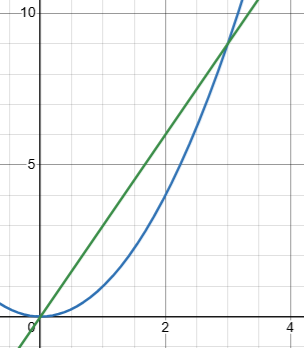
\includegraphics[width=0.5\linewidth]{1b.png}
    \caption{Región de integración b)}
    \label{fig:enter-label}
\end{figure}